\renewcommand\theequation{\arabic{chapter}.\arabic{section}.\arabic{equation}}
\setcounter{chapter}{14}
\chapter{Non-Abelian Gauge Invariance}
\setcounter{section}{2}
\section{The Gauge-Invariant Wilson Loop}
\subsection{(15.62)}
(15.56)を$\epsilon$の1次まで展開すれば,
\[
U_P(x, x) \approx 1 + ig \oint ds \, \frac{dx^\mu}{ds} A^a_\mu(x(s)) t^a
\approx 1 + ig \left[ \frac{\partial A_2^a}{\partial x^1} \epsilon^2 - \frac{\partial A_1^a}{\partial x^2} \epsilon^2 \right] t^a .
\]
2次の展開は
\begin{align*}
  & - \frac{g^2}{2} \int_0^1 ds_1 \int_0^1 ds_2 \, \frac{dx^\mu}{ds_1} \frac{dx^\nu}{ds_2}
  A^a_\mu(x(s_1)) A^b_\nu(x(s_1)) P \{ t^a t^b \} \\
  &\approx - \frac{g^2}{2} A^a_\mu(x) A^b_\nu(x)
  \int_0^1 ds_1 \int_0^1 ds_2 \, \frac{dx^\mu}{ds_1} \frac{dx^\nu}{ds_2} P \{ t^a t^b \}
\end{align*}
で与えられる.$s_1 > s_2$なら$P \{ t^a t^b \} = t^a t^b$である.

\begin{center}
  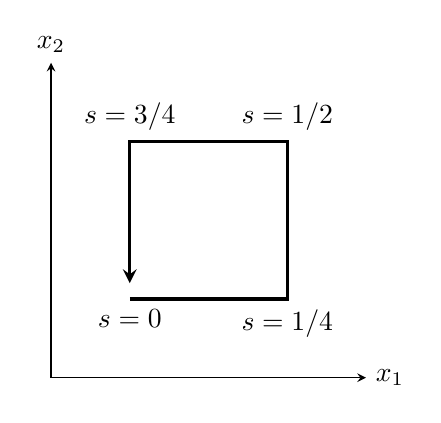
\begin{tikzpicture}[>=stealth]
    \draw[->] (0, 0) -- (4, 0) node [right] {$x_1$};
    \draw[->] (0, 0) -- (0, 4) node [above] {$x_2$};
    \draw[very thick, ->] (1, 1) node [below] {$s=0$} --
    (3, 1) node [below] {$s=1/4$} --
    (3, 3) node [above] {$s=1/2$} --
    (1, 3) node [above] {$s=3/4$} -- (1, 1.2);
  \end{tikzpicture}
\end{center}

$\mu = \nu = 1$の場合,$dx^1/ds \neq 0$となるのは$0 < s < 1/4$と$1/2 < s < 3/4$のみ.

\begin{center}
  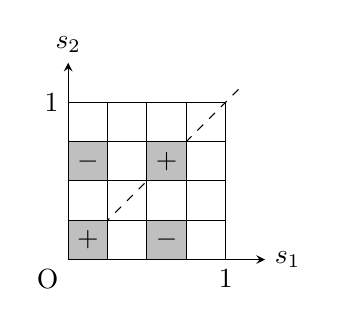
\begin{tikzpicture}[>=stealth]
    \draw[->] (0, 0) node [below left] {O} -- (2.5, 0) node [right] {$s_1$};
    \draw[->] (0, 0) -- (0, 2.5) node [above] {$s_2$};
    \draw (2, 0) node [below] {$1$};
    \draw (0, 2) node [left] {$1$};
    \draw[dashed] (0, 0) -- (2.2, 2.2);
    \foreach \i in {1, ..., 4}
      \draw (0, 0.5*\i) -- (2, 0.5*\i);
    \foreach \i in {1, ..., 4}
      \draw (0.5*\i, 0) -- (0.5*\i, 2);
    \filldraw[fill=lightgray] (0, 0) rectangle (0.5, 0.5);
    \draw (0.25, 0.25) node {$+$};
    \filldraw[fill=lightgray] (1, 0) rectangle (1.5, 0.5);
    \draw (1.25, 0.25) node {$-$};
    \filldraw[fill=lightgray] (0, 1) rectangle (0.5, 1.5);
    \draw (0.25, 1.25) node {$-$};
    \filldraw[fill=lightgray] (1, 1) rectangle (1.5, 1.5);
    \draw (1.25, 1.25) node {$+$};
  \end{tikzpicture}
\end{center}

$s_1 > s_2$の領域では積分が$0$になり,$s_1 < s_2$の領域でも同様に積分は$0$となる.

$\mu = \nu = 2$の場合,$dx^2/ds \neq 0$となるのは$1/4 < s < 1/2$と$3/4 < s < 1$のみ.
$s_1 > s_2$の領域では積分が$0$になり,$s_1 < s_2$の領域でも同様に積分は$0$となる.

$\mu =1$, $\nu = 2$の場合.

\begin{center}
  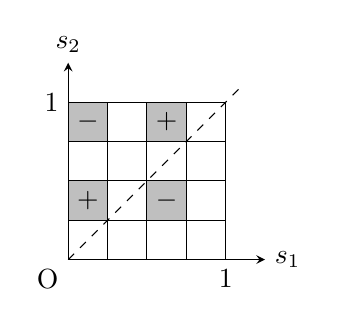
\begin{tikzpicture}[>=stealth]
    \draw[->] (0, 0) node [below left] {O} -- (2.5, 0) node [right] {$s_1$};
    \draw[->] (0, 0) -- (0, 2.5) node [above] {$s_2$};
    \draw (2, 0) node [below] {$1$};
    \draw (0, 2) node [left] {$1$};
    \draw[dashed] (0, 0) -- (2.2, 2.2);
    \foreach \i in {1, ..., 4}
      \draw (0, 0.5*\i) -- (2, 0.5*\i);
    \foreach \i in {1, ..., 4}
      \draw (0.5*\i, 0) -- (0.5*\i, 2);
    \filldraw[fill=lightgray] (0, 0.5) rectangle (0.5, 1);
    \draw (0.25, 0.75) node {$+$};
    \filldraw[fill=lightgray] (1, 0.5) rectangle (1.5, 1);
    \draw (1.25, 0.75) node {$-$};
    \filldraw[fill=lightgray] (0, 1.5) rectangle (0.5, 2);
    \draw (0.25, 1.75) node {$-$};
    \filldraw[fill=lightgray] (1, 1.5) rectangle (1.5, 2);
    \draw (1.25, 1.75) node {$+$};
  \end{tikzpicture}
\end{center}

$s_1 > s_2$の領域では積分は
\[ - 16\epsilon^2 \frac{1}{16} t^a t^b = - \epsilon^2 t^a t^b . \]
$s_1 > s_2$の領域では積分は
\[ + 16\epsilon^2 \frac{1}{16} t^b t^a = \epsilon^2 t^b t^a . \]
(15.44)から
\[ \epsilon^2 \frac{g^2}{2} A_1^a A_2^b [t^a, t^b] = \frac{i}{2} g^2 \epsilon^2 f^{abc} A_1^a A_2^b t^c . \]

$\mu = 2$, $\nu = 1$の場合も同様なので,
\begin{align*}
  U_P(x, x) &\approx
  1 + ig \left[ \frac{\partial A_2^a}{\partial x^1} \epsilon^2 - \frac{\partial A_1^a}{\partial x^2} \epsilon^2 \right] t^a + i g \epsilon^2 f^{abc} A_1^a A_2^b t^c \\
  &= 1 + ig\epsilon^2 \left[ \partial_1 A_2^c - \partial_2 A_1^c + g f^{abc} A_1^a A_2^b \right] t^c .
\end{align*}

\chapter{Quantization of Non-Abelian Gauge Theories}
\setcounter{section}{2}
\section{Ghosts and Unitarity}
\subsection{Figure 16.5}
\begin{center}
  \begin{tikzpicture}
    \begin{feynman}
      \vertex (o) at (0, 0);
      \vertex (A) at (90: 1.5) {\(A^b_\mu\)};
      \vertex (gout) at (210: 1.5) {\(c^a\)};
      \vertex (gin) at (330: 1.5) {\(\bar{c}^c\)};
      \diagram*{
        (gin) -- [ghost, momentum'=\(k\)] (o) -- [ghost, momentum=\(p\)] (gout),
        (A) -- [photon, momentum=\(q\)] (o)
      };
      \draw (o) node [below right] {\(c^c\)};
      \draw (o) node [above left] {\(\bar{c}^a\)};
    \end{feynman}
  \end{tikzpicture}
\end{center}

(16.32)から
\begin{align*}
  \mathcal{L}_\text{ghost} &= \bar{c}^a \left( -g\partial^\mu f^{abc} A^b_\mu \right) c^c + \cdots \\
  &= -gf^{abc} \bar{c}^a (\partial^\mu A^b_\mu) c^c - gf^{abc} \bar{c}^a A^b_\mu (\partial^\mu c^c) + \cdots \\
  &= -gf^{abc} \bar{c}^a (-iq^\mu A^b_\mu) c^c - gf^{abc} \bar{c}^a A^b_\mu (-ik^\mu c^c) + \cdots \\
  &= -gf^{abc} \bar{c}^a (-ip^\mu A^b_\mu) c^c + \cdots
\end{align*}
となるので,頂点は
\[ i\mathcal{L} \to -gf^{abc}p_\mu . \]

\setcounter{section}{4}
\section{One-Loop Divergences of Non-Abelian Gauge Theory}
\subsection{p.522最後の式}
フェルミオンは$d(r)$個のDiracスピノル$\psi_i$からなる:$\psi = (\psi_1 , \ldots, \psi_{d(r)})$.
Lie代数の生成子はサイズが$d(r) \times d(r)$の行列$d(G)$個の集合:$\set{t^a | 1 \leq a \leq d(G)}$.

(16.34)のうち,ボソンとフェルミオンの頂点は
\[ \mathcal{L}_{\bar\psi\psi A} = g \bar\psi^i \gamma^\mu \psi^j A_\mu^b (t^b)_{ij} \]
なので,
\[
\vcenter{\hbox{
\begin{tikzpicture}
  \begin{feynman}
    \vertex (o) at (0, 0);
    \vertex (a) at (90: 1.5) {$A^b_\mu$};
    \vertex (b) at (210: 1.5) {$\psi^i$};
    \vertex (c) at (330: 1.5) {$\bar\psi^j$};
    \diagram*{
    (o) -- [boson] (a);
    (c) -- [fermion] (o) -- [fermion] (b);
    };
    \draw (o) node [above right] {\(\psi^j\)};
    \draw (o) node [above left] {\(\bar\psi^i\)};
  \end{feynman}
\end{tikzpicture}
}}
= ig\gamma^\mu(t^b)_{ij}
\]
で与えられる.よって,
\begin{align*}
  \vcenter{\hbox{
  \begin{tikzpicture}
    \begin{feynman}
      \vertex (a) at (1.6, 0) {$b, \nu$};
      \vertex (b) at (0.7, 0);
      \vertex (c) at (-0.7, 0);
      \vertex (d) at (-1.6, 0) {$a, \mu$};
      \diagram*{
      (a) -- [boson] (b),
      (c) -- [boson] (d),
      (b) -- [fermion, half left, looseness=1.5, edge label=$p$, edge label'=$i$] (c),
      (c) -- [fermion, half left, looseness=1.5, edge label=$p+q$, edge label'=$j$] (b)
      };
    \end{feynman}
  \end{tikzpicture}
  }}
  &= - (ig)^2 \int \frac{d^dp}{(2\pi)^d} \Tr\left[ \gamma^\mu \frac{i}{\slashed{q}} \gamma^\nu \frac{i}{\slashed{p}+\slashed{q}} \right]
  (t^a)_{ji} (t^b)_{ij} \\[-20pt]
  &= - (ig)^2 \int \frac{d^dp}{(2\pi)^d} \Tr\left[ \gamma^\mu \frac{i}{\slashed{q}} \gamma^\nu \frac{i}{\slashed{p}+\slashed{q}} \right]
  \Tr [t^a t^b] .
\end{align*}

\subsection{(16.72)}
一般ゲージ(16.29)
\[
\wick{\c1{A}_\mu^a(p) \c1{A}_\nu^b(q)} = (2\pi)^4 \mathop{\delta^{(4)}}(p+q) \frac{-i}{p^2}
\left[ g_{\mu\nu} - (1-\xi) \frac{p_\mu p_\nu}{p^2} \right] \delta^{ab} .
\]
を使って計算する.

\subsubsection{(16.62)の修正}
(16.60)は
\begin{align*}
  \vcenter{\hbox{
  \begin{tikzpicture}
    \begin{feynman}
      \vertex (a) at (2, 0) {$b, \nu$};
      \vertex (b) at (1, 0);
      \vertex (c) at (-1, 0);
      \vertex (d) at (-2, 0) {$a, \mu$};
      \diagram*{
      (a) -- [boson] (b),
      (c) -- [boson] (d),
      (b) -- [boson, half right, looseness=1.5, reversed momentum=$p+q$] (c),
      (c) -- [boson, half right, looseness=1.5, reversed momentum=$p$] (b)
      };
    \end{feynman}
    \draw (c) + (-0.1, 0.8) node {$d, \sigma$};
    \draw (c) + (-0.1, -0.8) node {$c, \rho$};
    \draw (b) + (0.1, 0.8) node {$d, \sigma'$};
    \draw (b) + (0.1, -0.8) node {$c, \rho'$};
  \end{tikzpicture}
  }}
  &= \frac{1}{2} \int \frac{d^dp}{(2\pi)^d} \frac{-i}{p^2} \frac{-i}{(p+q)^2} g^2 f^{acd} f^{bcd} N^{\mu\nu}_\xi \\[-20pt]
  &= - \frac{g^2}{2} C_2(G) \delta^{ab} \int \frac{d^dp}{(2\pi)^d} \frac{1}{p^2(p+q)^2} N^{\mu\nu}_\xi
\end{align*}
となる.ただし,
\begin{align*}
  N^{\mu\nu}_\xi &=
  \left[ g_{\sigma\sigma'} - (1-\xi) \frac{(p+q)_\sigma (p+q)_{\sigma'}}{(p+q)^2} \right]
  \left[ g_{\rho\rho'} - (1-\xi) \frac{p_\rho p_{\rho'}}{p^2} \right] \\
  & \quad\times \left[ g^{\mu\rho} (q-p)^\sigma + g^{\rho\sigma} (2p+q)^\mu + g^{\sigma\mu} (-p-2q)^\rho \right] \\
  & \qquad\times \left[ g^{\nu\rho'} (p-q)^{\sigma'} + g^{\rho'\sigma'} (-2p-q)^\nu + g^{\sigma'\nu} (p+2q)^{\rho'} \right] \\
  %
  %
  &= N^{\mu\nu} \\
  & \quad - g_{\sigma\sigma'} (1-\xi) \frac{p_\rho p_{\rho'}}{p^2} [\cdots] [\cdots] \\
  & \quad - g_{\rho\rho'} (1-\xi) \frac{(p+q)_\sigma (p+q)_{\sigma'}}{(p+q)^2} [\cdots] [\cdots] \\
  & \quad + (1-\xi)^2 \frac{(p+q)_\sigma (p+q)_{\sigma'}}{(p+q)^2} \frac{p_\rho p_{\rho'}}{p^2} [\cdots] [\cdots] \\
  %
  %
  &= N^{\mu\nu} \\
  & \quad - \frac{1-\xi}{p^2} \left[ p^\mu (q-p)^\sigma + p^\sigma (2p+q)^\mu + g^{\sigma\mu} p \cdot (-p-2q) \right] \\
  & \qquad\times \left[ p^\nu (p-q)_\sigma + p_\sigma (-2p-q)^\nu + \delta^\nu{}_\sigma p \cdot (p+2q) \right] \\
  %
  & \quad - \frac{1-\xi}{(p+q)^2} \left[ g^{\mu\rho} (p+q) \cdot (q-p) + (p+q)^\rho (2p+q)^\mu + (p+q)^\mu (-p-2q)^\rho \right] \\
  & \qquad\times \left[ \delta^\nu{}_\rho (p+q) \cdot (p-q) + (p+q)_\rho (-2p-q)^\nu + (p+q)^\nu (p+2q)_\rho \right] \\
  %
  & \quad + \frac{(1-\xi)^2}{p^2(p+q)^2}
  \left[ p^\mu (p+q) \cdot (q-p) + p \cdot (p+q) (2p+q)^\mu + (p+q)^\mu p \cdot (-p-2q) \right] \\
  & \qquad\times \left[ p^\nu (p+q) \cdot (p-q) + p \cdot (p+q) (-2p-q)^\nu + (p+q)^\nu p \cdot (p+2q) \right] \\
  %
  %
  &= N^{\mu\nu} \\
  & \quad - \frac{1-\xi}{p^2} \left[ p^\mu (q-p)^\sigma + p^\sigma (2p+q)^\mu + g^{\sigma\mu} p \cdot (-p-2q) \right] \\
  & \qquad\times \left[ p^\nu (p-q)_\sigma + p_\sigma (-2p-q)^\nu + \delta^\nu{}_\sigma p \cdot (p+2q) \right] \\
  %
  & \quad - \frac{1-\xi}{(p+q)^2} \left[ (p+q)^\mu (-p-2q)^\sigma + (p+q)^\sigma (2p+q)^\mu + g^{\sigma\mu} (p+q) \cdot (q-p) \right] \\
  & \qquad\times \left[ (p+q)^\nu (p+2q)_\sigma + (p+q)_\sigma (-2p-q)^\nu + \delta^\nu{}_\sigma (p+q) \cdot (p-q) \right] \\
  %
  & \quad + \frac{(1-\xi)^2}{p^2(p+q)^2}
  \left[ p^\mu (p+q) \cdot (q-p) + p \cdot (p+q) (2p+q)^\mu + (p+q)^\mu p \cdot (-p-2q) \right] \\
  & \qquad\times \left[ p^\nu (p+q) \cdot (p-q) + p \cdot (p+q) (-2p-q)^\nu + (p+q)^\nu p \cdot (p+2q) \right] .
\end{align*}
ここで,第2項の$[\cdots][\cdots]$を$p \mapsto p+q$および$q \mapsto -q$とすれば第3項の$[\cdots][\cdots]$となる.さらに,
\[
\int \frac{d^dp}{(2\pi)^d} \frac{1}{p^4(p+q)^2} \mapsto \int \frac{d^dp}{(2\pi)^d} \frac{1}{(p+q)^4p^2}
\]
となるので,第2項と第3項の積分は等しい.

第4項を計算する.(6.42)より分母は
\begin{align*}
  \int \frac{d^dp}{(2\pi)^d} \frac{1}{p^4(p+q)^4}
  &= 6 \int_0^1 dx\,dy\, \delta(x+y-1) \int \frac{d^dp}{(2\pi)^d} \frac{xy}{[yp^2+x(p+q)^2]^4} \\
  &= 6 \int_0^1 dx \int \frac{d^dp}{(2\pi)^d} \frac{x(1-x)}{[(1-x)p^2+x(p+q)^2]^4} \\
  &= 6 \int_0^1 dx \int \frac{d^dP}{(2\pi)^d} \frac{x(1-x)}{[P^2 - \Delta]^4} \\
  & ( P = p + xq , \quad \Delta = - x(1-x) q^2 ) .
\end{align*}
分子は
\begin{align*}
  & p^\mu (p+q) \cdot (q-p) + p \cdot (p+q) (2p+q)^\mu + (p+q)^\mu p \cdot (-p-2q) \\
  & = p^\mu (q^2 - p^2) + (p^2 + p \cdot q) (2p+q)^\mu + (p+q)^\mu (-p^2 - 2p \cdot q) \\
  &= q^2 p^\mu - (p\cdot q) q^\mu
\end{align*}
及び
\begin{align*}
  & p^\nu (p+q) \cdot (p-q) + p \cdot (p+q) (-2p-q)^\nu + (p+q)^\nu p \cdot (p+2q) \\
  &= p^\nu (p^2 - q^2) + (p^2 + p \cdot q) (-2p-q)^\nu + (p+q)^\nu (p^2 + 2 p \cdot q) \\
  &= -q^2 p^\nu + (p\cdot q) q^\nu
\end{align*}
をかけて
\begin{align*}
  & [q^2 p^\mu - (p\cdot q) q^\mu][-q^2 p^\nu + (p\cdot q) q^\nu] \\
  & = - q^4 p^\mu p^\nu - (p\cdot q)^2 q^\mu q^\nu + q^2 (p\cdot q) (p^\mu q^\nu + q^\mu p^\nu) \\
  %
  &\to -q^4 \left[ P^\mu P^\nu + x^2 q^\mu q^\nu \right]
  - \left[ P \cdot q - xq^2 \right]^2 q^\mu q^\nu \\
  & \qquad + q^2 [ P \cdot q - xq^2 ] [P^\mu q^\nu + q^\mu P^\nu - 2xq^\mu q^\nu] \\
  %
  &\to -q^4 \left[ P^\mu P^\nu + x^2 q^\mu q^\nu \right]
  - \left[ (P \cdot q)^2 + x^2 q^4 \right] q^\mu q^\nu \\
  & \qquad + q^2 \left[ P^\rho q_\rho (P^\mu q^\nu + q^\mu P^\nu) + 2x^2 q^2 q^\mu q^\nu \right] \\
  %
  &= -q^4 P^\mu P^\nu - x^2 q^4 q^\mu q^\nu
  - \left[ (P \cdot q)^2 + x^2 q^4 \right] q^\mu q^\nu \\
  & \qquad + q^2 q^\nu q_\rho P^\mu P^\rho + q^2 q^\mu q_\rho P^\nu P^\rho + 2x^2 q^4 q^\mu q^\nu  \\
  %
  &= -q^4 P^\mu P^\nu
  - q_\rho q_\sigma q^\mu q^\nu P^\rho P^\sigma
  + q^2 q^\nu q_\rho P^\mu P^\rho + q^2 q^\mu q_\rho P^\nu P^\rho \\
  %
  &\to -q^4 \frac{g^{\mu\nu}}{d} P^2
  - q_\rho q_\sigma q^\mu q^\nu \frac{g^{\rho\sigma}}{d} P^2
  + q^2 q^\nu q_\rho \frac{g^{\mu\rho}}{d} P^2
  + q^2 q^\mu q_\rho \frac{g^{\nu\rho}}{d} P^2 \\
  %
  &= -q^4 \frac{g^{\mu\nu}}{d} P^2
  - q^2 q^\mu q^\nu \frac{1}{d} P^2
  + q^2 q^\nu q^\mu \frac{1}{d} P^2
  + q^2 q^\mu q^\nu \frac{1}{d} P^2 \\
  &= - (q^2 g^{\mu\nu} - q^\mu q^\nu) \frac{q^2}{d} P^2 .
\end{align*}
よって,第4項は
\begin{align}
   - 3 g^2 (1-\xi)^2 C_2(G) \delta^{ab} (q^2 g^{\mu\nu} - q^\mu q^\nu) \frac{q^2}{d} \int_0^1 dx \, x(1-x)
  \int \frac{d^dP}{(2\pi)^d} \frac{P^2}{[P^2 - \Delta]^4}
\end{align}
となる(有限値).

第2項(と第3項は等しい)を計算する.(6.40)から分母は
\begin{align*}
  & \int \frac{d^dp}{(2\pi)^d} \frac{1}{p^4(p+q)^2} \\
  &= \int_0^1 dx \, dy \, \delta(x+y-1) \int \frac{d^dp}{(2\pi)^d} \frac{2y}{[(1-x) p^2 + x (p+q)^2]^3} \\
  &= 2 \int_0^1 dx \, (1-x) \int \frac{d^dP}{(2\pi)^d} \frac{1}{[P^2 - \Delta]^3} , \\
  & ( P = p + xq , \quad \Delta = - x(1-x) q^2 ) .
\end{align*}
分子は
\begin{align*}
  & \left[ p^\mu (q-p)^\sigma + p^\sigma (2p+q)^\mu + g^{\sigma\mu} p \cdot (-p-2q) \right] \\
  & \times \left[ p^\nu (p-q)_\sigma + p_\sigma (-2p-q)^\nu + \delta^\nu{}_\sigma p \cdot (p+2q) \right] \\
  %
  &= - p^\mu p^\nu (q-p)^2 - g^{\mu\nu} (p^2 + 2p \cdot q)^2 - p^2 (q+2p)^\mu (q+2p)^\nu \\
  & \qquad % (2, 1) + (3, 1) + (3, 2)
  + p \cdot (p-q) (2p+q)^\mu p^\nu
  + p \cdot (p+2q) (q-p)^\mu p^\nu
  + p \cdot (p+2q) p^\mu (2p+q)^\nu \\
  & \qquad + (\!( \mu\leftrightarrow\nu )\!) \\
  %
  &= - (P^\mu - xq^\mu)(P^\nu - xq^\nu) [P - (x+1)q]^2 \\
  &\quad - g^{\mu\nu} \left[ (P - xq)^2 + 2(P - xq) \cdot q \right]^2 \\
  &\quad - (P-xq)^2 (2P + (1-2x)q)^\mu (2P + (1-2x)q)^\nu \\
  &\qquad + (P-xq) \cdot (P - (x+1)q) (2P + (1-2x)q)^\mu (P-xq)^\nu \\
  &\qquad + (P-xq) \cdot (P + (2-x)q) (-P+(x+1)q)^\mu (P-xq)^\nu \\
  &\qquad + (P-xq) \cdot (P + (2-x)q) (P-xq)^\mu (2P + (1-2x)q)^\nu \\
  &\qquad + (\!( \mu\leftrightarrow\nu )\!) \\
  %
  &\to - (P^\mu P^\nu - x P^\mu q^\nu - x q^\mu P^\nu + x^2 q^\mu q^\nu) \left[ P^2 - 2(x+1)P \cdot q + (x+1)^2 q^2 \right] \\
  &\quad - g^{\mu\nu} \left[ P^2 - 2(x-1) P \cdot q + x(x-2) q^2 \right]^2 \\
  &\quad - (P^2 - 2x P \cdot q + x^2q^2) [4P^\mu P^\nu +2(1-2x) (P^\mu q^\nu + q^\mu P^\nu) + (1-2x)^2 q^\mu q^\nu] \\
  &\qquad + (P^2 - (2x+1) P \cdot q + x(x+1) q^2)
  (2P^\mu P^\nu - 2xP^\mu q^\nu + (1-2x) q^\mu P^\nu - x(1-2x) q^\mu q^\nu) \\
  &\qquad + (P^2 + 2(1-x) P \cdot q - x(2-x) q^2)
  (-P^\mu P^\nu + x P^\mu q^\nu + (x+1) q^\mu P^\nu - x(x+1) q^\mu q^\nu) \\
  &\qquad + (P^2 + 2(1-x) P \cdot q - x(2-x) q^2)
  (2P^\mu P^\nu + (1-2x) P^\mu q^\nu - 2x q^\mu P^\nu  - x(1-2x) q^\mu q^\nu) \\
  &\qquad + (\!( \mu\leftrightarrow\nu )\!) \\
  %
  &\to - P^2 P^\mu P^\nu - (x+1)^2 q^2 P^\mu P^\nu - x^2 q^\mu q^\nu P^2 \\
  &\qquad - x^2(x+1)^2 q^2 q^\mu q^\nu - 2x(x+1) q_\rho P^\rho (P^\mu q^\nu + q^\mu P^\nu) \\
  &\quad - g^{\mu\nu} \left[ (P^2)^2 + 4(x-1)^2 q_\rho q_\sigma P^\rho P^\sigma + 2x(x-2) q^2 P^2 + x^2(x-2)^2 q^4 \right] \\
  &\quad - 4P^2 P^\mu P^\nu - 4x^2 q^2 P^\mu P^\nu - (1-2x)^2 q^\mu q^\nu P^2 \\
  &\qquad - x^2 (1-2x)^2 q^2 q^\mu q^\nu + 4x(1-2x) q_\rho P^\rho (P^\mu q^\nu + q^\mu P^\nu) \\
  &\quad + (P^2 - (2x+1) P \cdot q + x(x+1) q^2)
  [4P^\mu P^\nu + (1-4x) (P^\mu q^\nu + q^\mu P^\nu) - 2x(1-2x) q^\mu q^\nu] \\
  &\quad + (P^2 + 2(1-x) P \cdot q - x(2-x) q^2)
  [-2P^\mu P^\nu + (2x+1) (P^\mu q^\nu + q^\mu P^\nu) - 2x(x+1) q^\mu q^\nu] \\
  &\quad + (P^2 + 2(1-x) P \cdot q - x(2-x) q^2)
  [4P^\mu P^\nu + (1-4x) (P^\mu q^\nu + q^\mu P^\nu) - 2x(1-2x) q^\mu q^\nu] \\
  %
  &= - P^2 P^\mu P^\nu - (x+1)^2 q^2 P^\mu P^\nu - x^2 q^\mu q^\nu P^2 \\
  &\qquad - x^2(x+1)^2 q^2 q^\mu q^\nu - 2x(x+1) q_\rho P^\rho (P^\mu q^\nu + q^\mu P^\nu) \\
  &\quad - g^{\mu\nu} \left[ (P^2)^2 + 4(x-1)^2 q_\rho q_\sigma P^\rho P^\sigma + 2x(x-2) q^2 P^2 + x^2(x-2)^2 q^4 \right] \\
  &\quad - 4P^2 P^\mu P^\nu - 4x^2 q^2 P^\mu P^\nu - (1-2x)^2 q^\mu q^\nu P^2 \\
  &\qquad - x^2 (1-2x)^2 q^2 q^\mu q^\nu + 4x(1-2x) q_\rho P^\rho (P^\mu q^\nu + q^\mu P^\nu) \\
  &\quad + (2P^2 + (1 - 4x) P \cdot q + x(2x-1) q^2)
  [4P^\mu P^\nu + (1-4x) (P^\mu q^\nu + q^\mu P^\nu) - 2x(1-2x) q^\mu q^\nu] \\
  &\quad + (P^2 + 2(1-x) P \cdot q - x(2-x) q^2)
  [-2P^\mu P^\nu + (2x+1) (P^\mu q^\nu + q^\mu P^\nu) - 2x(x+1) q^\mu q^\nu] \\
  %
  &\to - P^2 P^\mu P^\nu - (x+1)^2 q^2 P^\mu P^\nu - x^2 q^\mu q^\nu P^2 \\
  &\qquad - x^2(x+1)^2 q^2 q^\mu q^\nu - 2x(x+1) q_\rho P^\rho (P^\mu q^\nu + q^\mu P^\nu) \\
  &\quad - g^{\mu\nu} \left[ (P^2)^2 + 4(x-1)^2 q_\rho q_\sigma P^\rho P^\sigma + 2x(x-2) q^2 P^2 + x^2(x-2)^2 q^4 \right] \\
  &\quad - 4P^2 P^\mu P^\nu - 4x^2 q^2 P^\mu P^\nu - (1-2x)^2 q^\mu q^\nu P^2 \\
  &\qquad - x^2 (1-2x)^2 q^2 q^\mu q^\nu + 4x(1-2x) q_\rho P^\rho (P^\mu q^\nu + q^\mu P^\nu) \\
  &\quad + 8 P^2 P^\mu P^\nu + 4x(2x-1)q^2 P^\mu P^\nu - 4x(1-2x) q^\mu q^\nu P^2 \\
  & \qquad + 2x^2(1-2x)^2 q^2 q^\mu q^\nu + (1-4x)^2 q_\rho P^\rho (P^\mu q^\nu + q^\mu P^\nu) \\
  &\quad -2 P^2 P^\mu P^\nu + 2x(2-x)q^2 P^\mu P^\nu - 2x(x+1) q^\mu q^\nu P^2 \\
  & \qquad + 2x^2(2-x)(x+1) q^2 q^\mu q^\nu + 2(1-x)(2x+1) q_\rho P^\rho (P^\mu q^\nu + q^\mu P^\nu) \\
  %
  &= - g^{\mu\nu} \left[ (P^2)^2 + 4(x-1)^2 q_\rho q_\sigma P^\rho P^\sigma + 2x(x-2) q^2 P^2 + x^2(x-2)^2 q^4 \right] \\
  &\quad - P^2 P^\mu P^\nu - (x+1)^2 q^2 P^\mu P^\nu - x^2 q^\mu q^\nu P^2 \\
  &\qquad - x^2(x+1)^2 q^2 q^\mu q^\nu - 2x(x+1) q_\rho P^\rho (P^\mu q^\nu + q^\mu P^\nu) \\
  &\quad - 4P^2 P^\mu P^\nu - 4x^2 q^2 P^\mu P^\nu - (1-2x)^2 q^\mu q^\nu P^2 \\
  &\qquad - x^2 (1-2x)^2 q^2 q^\mu q^\nu + 4x(1-2x) q_\rho P^\rho (P^\mu q^\nu + q^\mu P^\nu) \\
  &\quad + 8 P^2 P^\mu P^\nu + 4x(2x-1)q^2 P^\mu P^\nu - 4x(1-2x) q^\mu q^\nu P^2 \\
  & \qquad + 2x^2(1-2x)^2 q^2 q^\mu q^\nu + (1-4x)^2 q_\rho P^\rho (P^\mu q^\nu + q^\mu P^\nu) \\
  &\quad -2 P^2 P^\mu P^\nu + 2x(2-x)q^2 P^\mu P^\nu - 2x(x+1) q^\mu q^\nu P^2 \\
  & \qquad + 2x^2(2-x)(x+1) q^2 q^\mu q^\nu + 2(1-x)(2x+1) q_\rho P^\rho (P^\mu q^\nu + q^\mu P^\nu) \\
  %
  &= - g^{\mu\nu} \left[ (P^2)^2 + 4(x-1)^2 q_\rho q_\sigma P^\rho P^\sigma + 2x(x-2) q^2 P^2 + x^2(x-2)^2 q^4 \right] \\
  &\quad + P^2 P^\mu P^\nu + (x^2-2x-1) q^2 P^\mu P^\nu + (x^2-2x-1) q^\mu q^\nu P^2 \\
  &\qquad + x^2 (x-2)^2 q^2 q^\mu q^\nu + (2x^2-4x+3) q_\rho P^\rho (P^\mu q^\nu + q^\mu P^\nu) \\
  %
  &\to - g^{\mu\nu} \left[ (P^2)^2 + 4(x-1)^2 q_\rho q_\sigma \frac{g^{\rho\sigma}}{d} P^2 + 2x(x-2) q^2 P^2 + x^2(x-2)^2 q^4 \right] \\
  &\quad + P^2 P^\mu P^\nu + (x^2-2x-1) q^2 \frac{g^{\mu\nu}}{d} P^2 + (x^2-2x-1) q^\mu q^\nu P^2 \\
  &\qquad + x^2 (x-2)^2 q^2 q^\mu q^\nu + (2x^2-4x+3) q_\rho \left( q^\nu \frac{g^{\mu\rho}}{d} P^2 + q^\mu \frac{g^{\nu\rho}}{d} P^2 \right) \\
  %
  &= - g^{\mu\nu} \left[ (P^2)^2 + \left\{ \frac{4}{d}(x-1)^2 + 2x(x-2) \right\} q^2 P^2 + x^2(x-2)^2 q^4 \right] \\
  &\quad + P^2 P^\mu P^\nu + (x^2-2x-1) q^2 \frac{g^{\mu\nu}}{d} P^2 + (x^2-2x-1) q^\mu q^\nu P^2 \\
  &\qquad + x^2 (x-2)^2 q^2 q^\mu q^\nu + \frac{2}{d} (2x^2-4x+3) q^\mu q^\nu P^2 \\
  %
  &= P^2 P^\mu P^\nu - g^{\mu\nu} (P^2)^2 - g^{\mu\nu} \left\{ \frac{1}{d}(3x^2-6x+5) + 2x(x-2) \right\} q^2 P^2 \\
  & \quad + \left\{ \frac{2}{d} (2x^2-4x+3) + (x^2-2x-1) \right\} q^\mu q^\nu P^2 - x^2(x-2)^2 q^2 (g^{\mu\nu}q^2 - q^\mu q^\nu) .
\end{align*}
最後の項は積分すれば有限値
\begin{align}
  2 g^2 (1-\xi) C_2(G) \delta^{ab} (g^{\mu\nu}q^2 - q^\mu q^\nu) \int_0^1 dx \, (1-x) \int \frac{d^dP}{(2\pi)^d} \frac{- x^2(x-2)^2 q^2}{[P^2-\Delta]^3}
\end{align}
になるので,これ以降は考えない.

以上から(16.62)に加わる発散項は
\begin{align}
  \begin{split}
    & 2 g^2 (1-\xi) C_2(G) \delta^{ab} \int_0^1 dx \,(1-x) \int \frac{d^dP}{(2\pi)^d} \frac{1}{[P^2-\Delta]^3} \\
    &\quad \times \left[ P^2 P^\mu P^\nu - g^{\mu\nu} (P^2)^2 - g^{\mu\nu} \left\{ \frac{1}{d}(3x^2-6x+5) + 2x(x-2) \right\} q^2 P^2 \right. \\
    &\qquad \left. + \left\{ \frac{2}{d} (2x^2-4x+3)+ (x^2-2x-1) \right\} q^\mu q^\nu P^2 \right]
   \end{split}
   \label{eq_17_72_modify_16_62_second_third_term_except_last}
\end{align}

\subsubsection{(16.65)の修正}
(16.63)は
\begin{align*}
  &
  \vcenter{\hbox{
  \begin{tikzpicture}[every loop/.style={min distance=25mm}]
    \begin{feynman}
      \vertex (o) at (0, 0) {$a, \mu$};
      \vertex (a) at (1.5, 0);
      \vertex (b) at (3, 0) {$b, \nu$};
      \diagram*{
      (o) -- [boson, momentum'=$q$] (a) -- [boson] (b)
      };
      \draw (a) edge [in=140, out=40, loop, boson, momentum'={[arrow shorten=0.3]$p$}] ();
    \end{feynman}
    \draw (a) + (0.8, 0.5) node {$c, \rho$};
    \draw (a) + (-0.8, 0.5) node {$d, \sigma$};
  \end{tikzpicture}
  }} \\
  &= \frac{1}{2} \int \frac{d^dp}{(2\pi)^d} \frac{-i}{p^2}
  \left[ g_{\rho\sigma} - (1-\xi) \frac{p_\rho p_\sigma}{p^2} \right] \delta^{cd} (-ig^2) \\
  & \quad \times \left[
  f^{abe} f^{cde} (g^{\mu\rho} g^{\nu\sigma} - g^{\mu\sigma} g^{\nu\rho})
  + f^{ace} f^{bde} (g^{\mu\nu} g^{\rho\sigma} - g^{\mu\sigma} g^{\nu\rho})
  + f^{ade} f^{bce} (g^{\mu\nu} g^{\rho\sigma} - g^{\mu\rho} g^{\nu\sigma})
  \right] \\
  %
  &= (16.65) + \frac{g^2}{2} (1-\xi) \int \frac{d^dp}{(2\pi)^d} \frac{p_\rho p_\sigma}{p^4} \delta^{cd} \\
  & \quad \times \left[
  f^{abe} f^{cde} (g^{\mu\rho} g^{\nu\sigma} - g^{\mu\sigma} g^{\nu\rho})
  + f^{ace} f^{bde} (g^{\mu\nu} g^{\rho\sigma} - g^{\mu\sigma} g^{\nu\rho})
  + f^{ade} f^{bce} (g^{\mu\nu} g^{\rho\sigma} - g^{\mu\rho} g^{\nu\sigma})
  \right] \\
  %
  &= (16.65) + \frac{g^2}{2} (1-\xi) \int \frac{d^dp}{(2\pi)^d} \frac{p_\rho p_\sigma}{p^4} f^{ace} f^{bce}
  \left[ g^{\mu\nu} g^{\rho\sigma} - g^{\mu\sigma} g^{\nu\rho}
  + g^{\mu\nu} g^{\rho\sigma} - g^{\mu\rho} g^{\nu\sigma} \right] \\
  %
  &= (16.65) + g^2 (1-\xi) C_2(G) \delta^{ab} \int \frac{d^dp}{(2\pi)^d} \frac{1}{p^4}
  \left[ g^{\mu\nu} p^2 - p^\mu p^\nu \right] \\
  %
  &= (16.65)
  + g^2 (1-\xi) C_2(G) \delta^{ab} \int \frac{d^dp}{(2\pi)^d} \frac{g^{\mu\nu}p^2}{p^4}
  - g^2 (1-\xi) C_2(G) \delta^{ab} \int \frac{d^dp}{(2\pi)^d} \frac{p^\mu p^\nu}{p^4} .
\end{align*}
第2項の積分は
\begin{align*}
  & \int \frac{d^dp}{(2\pi)^d} \frac{p^2}{p^4} \\
  &= \int \frac{d^dp}{(2\pi)^d} \frac{p^2}{p^4} \frac{(p+q)^2}{(p+q)^2} \\
  &= 2 \int_0^1 dx \, (1-x) \int \frac{d^dp}{(2\pi)^d} \frac{p^2 (p+q)^2}{[P^2-\Delta]^3} \\
  &= 2 \int_0^1 dx \, (1-x) \int \frac{d^dp}{(2\pi)^d} \frac{(P-xq)^2 (P+(1-x)q)^2}{[P^2-\Delta]^3} \\
  &= 2 \int_0^1 dx \, (1-x) \int \frac{d^dp}{(2\pi)^d} \frac{1}{[P^2-\Delta]^3} \\
  &\qquad\times \left[ P^2 - 2x P\cdot q + x^2 q^2 \right]
  \left[ P^2 + 2(1-x) P\cdot q + (1-x)^2 q^2 \right] \\
  %
  &\to 2 \int_0^1 dx \, (1-x) \int \frac{d^dp}{(2\pi)^d} \frac{1}{[P^2-\Delta]^3} \\
  &\qquad\times \left[ (P^2)^2 + (2x^2-2x+1) q^2 P^2 - 4x(1-x) q_\rho q_\sigma P^\rho P^\sigma + x^2(1-x)^2 q^4 \right] \\
  %
  &\to 2 \int_0^1 dx \, (1-x) \int \frac{d^dp}{(2\pi)^d} \frac{1}{[P^2-\Delta]^3} \\
  &\qquad\times \left[ (P^2)^2 + (2x^2-2x+1) q^2 P^2 - 4x(1-x) q_\rho q_\sigma \frac{g^{\rho\sigma}}{d} P^2 + x^2(1-x)^2 q^4 \right] \\
  %
  &\to 2 \int_0^1 dx \, (1-x) \int \frac{d^dp}{(2\pi)^d} \frac{1}{[P^2-\Delta]^3} \\
  &\qquad\times \left[ (P^2)^2 + \left\{ (2x^2-2x+1) - \frac{4}{d} x(1-x) \right\} q^2 P^2 + x^2(1-x)^2 q^4 \right] .
\end{align*}
第3項の積分は
\begin{align*}
  & \int \frac{d^dp}{(2\pi)^d} \frac{p^\mu p^\nu}{p^4} \\
  &= \int \frac{d^dp}{(2\pi)^d} \frac{p^\mu p^\nu}{p^4} \frac{(p+q)^2}{(p+q)^2} \\
  &= 2 \int_0^1 dx \, (1-x) \int \frac{d^dp}{(2\pi)^d} \frac{p^\mu p^\nu (p+q)^2}{[P^2-\Delta]^3} \\
  &= 2 \int_0^1 dx \, (1-x) \int \frac{d^dp}{(2\pi)^d} \frac{(P-xq)^\mu (P-xq)^\nu (P+(1-x)q)^2}{[P^2-\Delta]^3} \\
  &= 2 \int_0^1 dx \, (1-x) \int \frac{d^dp}{(2\pi)^d} \frac{1}{[P^2-\Delta]^3} \\
  &\qquad\times \left[ P^\mu P^\nu - x(P^\mu q^\nu+q^\mu P^\nu) + x^2 q^\mu q^\nu \right]
  [P^2 + 2(1-x)q \cdot P + (1-x)^2 q^2]  \\
  %
  &\to 2 \int_0^1 dx \, (1-x) \int \frac{d^dp}{(2\pi)^d} \frac{1}{[P^2-\Delta]^3} \\
  &\quad\times \bigl[ P^2 P^\mu P^\nu + (1-x)^2 q^2 P^\mu P^\nu + x^2 q^\mu q^\nu P^2 \\
  & \qquad + x^2(1-x)^2 q^\mu q^\nu q^2 - 2x(1-x) q_\rho P^\rho (P^\mu q^\nu+q^\mu P^\nu) \bigr] \\
  %
  &\to 2 \int_0^1 dx \, (1-x) \int \frac{d^dp}{(2\pi)^d} \frac{1}{[P^2-\Delta]^3} \\
  &\quad\times \left[ P^2 P^\mu P^\nu + (1-x)^2 q^2 \frac{g^{\mu\nu}}{d} P^2 + x^2 q^\mu q^\nu P^2 \right. \\
  & \qquad \left. + x^2(1-x)^2 q^\mu q^\nu q^2 - 2x(1-x) q_\rho \left( q^\nu \frac{g^{\mu\rho}}{d} P^2 + q^\mu \frac{g^{\nu\rho}}{d} P^2 \right) \right] \\
  %
  &= 2 \int_0^1 dx \, (1-x) \int \frac{d^dp}{(2\pi)^d} \frac{1}{[P^2-\Delta]^3} \\
  &\quad\times \left[ P^2 P^\mu P^\nu + (1-x)^2 q^2 \frac{g^{\mu\nu}}{d} P^2 + x^2 q^\mu q^\nu P^2
  + x^2(1-x)^2 q^\mu q^\nu q^2 - \frac{4}{d}x(1-x) q^\mu q^\nu P^2 \right] \\
  %
  &\to 2 \int_0^1 dx \, (1-x) \int \frac{d^dp}{(2\pi)^d} \frac{1}{[P^2-\Delta]^3} \\
  &\quad\times \left[ P^2 P^\mu P^\nu + g^{\mu\nu} \frac{1}{d} (1-x)^2 q^2 P^2
  + \left\{ x^2 - \frac{4}{d}x(1-x) \right\} q^\mu q^\nu P^2
  + x^2(1-x)^2 q^\mu q^\nu q^2 \right] .
\end{align*}
以上から(16.65)に加わる項は
\begin{align*}
  & 2 g^2 (1-\xi) C_2(G) \delta^{ab} \int_0^1 dx \, (1-x) \int \frac{d^dp}{(2\pi)^d} \frac{1}{[P^2-\Delta]^3} \\
  &\quad\times \left[ g^{\mu\nu} (P^2)^2 + g^{\mu\nu} \left\{ (2x^2-2x+1) - \frac{4}{d} x(1-x) \right\} q^2 P^2 + g^{\mu\nu} x^2(1-x)^2 q^4 \right] \\
  & - 2 g^2 (1-\xi) C_2(G) \delta^{ab} \int_0^1 dx \, (1-x) \int \frac{d^dp}{(2\pi)^d} \frac{1}{[P^2-\Delta]^3} \\
  &\quad\times \left[ P^2 P^\mu P^\nu + g^{\mu\nu} \frac{1}{d} (1-x)^2 q^2 P^2
  + \left\{ x^2 - \frac{4}{d}x(1-x) \right\} q^\mu q^\nu P^2
  + x^2(1-x)^2 q^\mu q^\nu q^2 \right] \\
  %
  &= 2 g^2 (1-\xi) C_2(G) \delta^{ab} \int_0^1 dx \, (1-x) \int \frac{d^dp}{(2\pi)^d} \frac{1}{[P^2-\Delta]^3} \\
  &\quad\times \left[ - P^2 P^\mu P^\nu + g^{\mu\nu} (P^2)^2 + g^{\mu\nu} \left\{ (2x^2-2x+1) + \frac{1}{d} (3x^2-2x-1) \right\} q^2 P^2 \right. \\
  &\qquad \left. - \left\{ x^2 - \frac{4}{d}x(1-x) \right\} q^\mu q^\nu P^2 + x^2(1-x)^2 q^2 (q^2g^{\mu\nu}-q^\mu q^\nu) \right] .
\end{align*}
最後の項
\begin{align}
  2 g^2 (1-\xi) C_2(G) \delta^{ab} (q^2g^{\mu\nu}-q^\mu q^\nu) \int_0^1 dx \, (1-x)
  \int \frac{d^dp}{(2\pi)^d} \frac{x^2(1-x)^2 q^2 }{[P^2-\Delta]^3}
\end{align}
は有限なので,これ以降考えない.以上から,(16.65)に加わる発散項は
\begin{align}
  \begin{split}
    & 2 g^2 (1-\xi) C_2(G) \delta^{ab} \int_0^1 dx \, (1-x) \int \frac{d^dp}{(2\pi)^d} \frac{1}{[P^2-\Delta]^3} \\
    &\quad\times \left[ - P^2 P^\mu P^\nu + g^{\mu\nu} (P^2)^2 + g^{\mu\nu} \left\{ (2x^2-2x+1) + \frac{1}{d} (3x^2-2x-1) \right\} q^2 P^2 \right. \\
    &\qquad \left. - \left\{ x^2 - \frac{4}{d}x(1-x) \right\} q^\mu q^\nu P^2 \right] .
  \end{split}
  \label{eq_17_72_modify_16_65}
\end{align}

\eqref{eq_17_72_modify_16_62_second_third_term_except_last}と\eqref{eq_17_72_modify_16_65}を足して,ゲージによる修正(のうち発散する部分)は
\begin{align*}
  & 2 g^2 (1-\xi) C_2(G) \delta^{ab} \int_0^1 dx \, (1-x) \int \frac{d^dP}{(2\pi)^d} \frac{1}{[P^2-\Delta]^3} \\
  &\quad \times \left[ P^2 P^\mu P^\nu - g^{\mu\nu} (P^2)^2 - g^{\mu\nu} \left\{ \frac{1}{d}(3x^2-6x+5) + 2x(x-2) \right\} q^2 P^2 \right. \\
  &\qquad\qquad \left. + \left\{ \frac{2}{d} (2x^2-4x+3) + (x^2-2x-1) \right\} q^\mu q^\nu P^2 \right] \\
  &+ 2 g^2 (1-\xi) C_2(G) \delta^{ab} \int_0^1 dx \, (1-x) \int \frac{d^dp}{(2\pi)^d} \frac{1}{[P^2-\Delta]^3} \\
  &\quad\times \left[ - P^2 P^\mu P^\nu + g^{\mu\nu} (P^2)^2 + g^{\mu\nu} \left\{ (2x^2-2x+1) + \frac{1}{d} (3x^2-2x-1) \right\} q^2 P^2 \right. \\
  &\qquad\qquad \left. - \left\{ x^2 - \frac{4}{d}x(1-x) \right\} q^\mu q^\nu P^2 \right] \\
  %
  &= 2 g^2 (1-\xi) C_2(G) \delta^{ab} \int_0^1 dx \, (1-x) \int \frac{d^dP}{(2\pi)^d} \frac{1}{[P^2-\Delta]^3} \\
  &\quad\times \left[ g^{\mu\nu} \left\{ (2x+1) + \frac{2}{d} (2x-3) \right\} q^2 P^2
  - \left\{ (2x+1) + \frac{2}{d}(2x-3) \right\} q^\mu q^\nu P^2 \right] \\
  %
  &= 2 g^2 (1-\xi) C_2(G) \delta^{ab} (q^2g^{\mu\nu} - q^\mu q^\nu) \int_0^1 dx \, (1-x)
  \left\{ (2x+1) + \frac{2}{d} (2x-3) \right\} \\
  &\quad\times \int \frac{d^dP}{(2\pi)^d} \frac{P^2}{[P^2-\Delta]^3} \\
  %
  &= 2 g^2 (1-\xi) C_2(G) \delta^{ab} (q^2g^{\mu\nu} - q^\mu q^\nu) \int_0^1 dx \, (1-x)
  \left\{ (2x+1) + \frac{2}{d} (2x-3) \right\} \\
  &\quad\times \frac{i}{(4\pi)^{d/2}} \frac{d}{2} \frac{\Gamma(2-d/2)}{\Gamma(3)} \left( \frac{1}{\Delta} \right)^{2-d/2} \\
  %
  &= \frac{2ig^2}{(4\pi)^{d/2}} (1-\xi) C_2(G) \delta^{ab} (q^2g^{\mu\nu} - q^\mu q^\nu) \\
  & \quad\times \int_0^1 dx \, (1-x) \left\{ (2x+1) + \frac{2}{d} (2x-3) \right\} \frac{\Gamma(2-d/2)}{\Delta^{2-d/2}} \\
  %
  &\approx
  i (q^2g^{\mu\nu} - q^\mu q^\nu) \delta^{ab} \left[ \frac{-g^2}{(4\pi)^2} \frac{-1+\xi}{2} C_2(G)\Gamma(2-d/2) \right] .
\end{align*}
(16.71)と比べて
\[ - \frac{5}{3} \mapsto - \frac{5}{3} + \frac{-1+\xi}{2} = - \frac{13}{6} + \frac{\xi}{2} \]
とすれば良いことが分かる.

\subsection{(16.88)}
(10.36)の直前で定義したように,
\[ \psi_0 = \sqrt{Z_2} \psi , \quad A^\mu_0 = \sqrt{Z_3} A^\mu . \]
(16.86)の第2項は
\[
\bar\psi_0 (i\slashed\partial - m_0) \psi_0 = Z_2 \bar\psi (i\slashed\partial - m_0) \psi
= \bar\psi (i\slashed\partial - m) \psi + \bar\psi (i\delta_2\slashed\partial - \delta_m) \psi .
\]
右辺の第1項は(16.34),第2項は(16.87)に含まれる.他も同様.

\section{Asymptotic Freedom: The Background Field Method}
\subsection{(16.99)}
ラグランジアン(16.98)が不変なことを確かめる.随伴表現$(t^b)_{ac} = i f^{abc}$を使う.
\[
\tilde{A}_\mu^a = A_\mu^a + \mathcal{A}_\mu^a , \quad
\tilde{D}_\mu^{ac} = D_\mu^{ac} + f^{abc}\mathcal{A}_\mu^b = \partial_\mu\delta^{ac} + f^{abc}\tilde{A}_\mu^b
\]
とする.$\tilde{A}_\mu^a$の変換は
\begin{align*}
  \tilde{A}_\mu^a &\to A_\mu^a + \mathcal{A}_\mu^a + (D_\mu \beta)^a - f^{abc} \beta^b \mathcal{A}_\mu^c \\
  &= A_\mu^a + \mathcal{A}_\mu^a + D_\mu^{ac} \beta^c - f^{acb} \beta^c \mathcal{A}_\mu^b \\
  &= A_\mu^a + \mathcal{A}_\mu^a + (\partial_\mu\delta^{ac} + f^{abc}A_\mu^b) \beta^c + f^{abc} \beta^c \mathcal{A}_\mu^b \\
  &= A_\mu^a + \mathcal{A}_\mu^a + (\partial_\mu\delta^{ac} + f^{abc}A_\mu^b + f^{abc}\mathcal{A}_\mu^b) \beta^c \\
  &= \tilde{A}_\mu^a + (\partial_\mu\delta^{ac} + f^{abc}\tilde{A}_\mu^b) \beta^c \\
  &= \tilde{A}_\mu^a + \tilde{D}_\mu^{ac} \beta^c \\
  &= \tilde{A}_\mu^a + (\tilde{D}_\mu \beta)^a \\
  &= \tilde{A}_\mu^a + \partial_\mu\beta^a + f^{abc}\tilde{A}_\mu^b \beta^c .
\end{align*}

\subsubsection{fermion}
フェルミオンの変換は
\[
\psi^a \to \psi^a + i \beta^b (t^b\psi)_a = \psi^a + i \beta^b (t^b)_{ac}\psi^c
= \psi^a - f^{abc} \beta^b \psi^c .
\]
(15.30)と同様にフェルミオンの共変微分はフェルミオンと同じ変換になる.実際,
\begin{align*}
  (\tilde{D}_\mu\psi)^a &= \tilde{D}_\mu^{ac} \psi^c \\
  &= (\partial_\mu\delta^{ac} + f^{abc}\tilde{A}_\mu^b) \psi^c \\
  &= \partial_\mu \psi^a + f^{abc}\tilde{A}_\mu^b \psi^c \\
  %
  &\to \partial_\mu (\psi^a - f^{abc} \beta^b \psi^c)
  + f^{abc} (\tilde{A}_\mu^b + \partial_\mu\beta^b + f^{bde}\tilde{A}_\mu^d\beta^e)
  (\psi^c - f^{cfg}\beta^f\psi^g) \\
  %
  &\approx \partial_\mu \psi^a - f^{abc}(\partial_\mu\beta^b)\psi^c - f^{abc} \beta^b \partial_\mu\psi^c\\
  &\quad + f^{abc} \left[ \tilde{A}_\mu^b \psi^c + (\partial_\mu\beta^b)\psi^c
  + f^{bde}\tilde{A}_\mu^d\beta^e\psi^c - \tilde{A}_\mu^b f^{cfg}\beta^f\psi^g \right] \\
  %
  &= \partial_\mu \psi^a - f^{abc} \beta^b \partial_\mu\psi^c
  + f^{abc} \left[ \tilde{A}_\mu^b \psi^c
  + f^{bde}\tilde{A}_\mu^d\beta^e\psi^c - \tilde{A}_\mu^b f^{cfg}\beta^f\psi^g \right] \\
  %
  &= \partial_\mu \psi^a + f^{abc} \tilde{A}_\mu^b \psi^c - f^{abc} \beta^b \partial_\mu\psi^c
  + f^{abc} f^{bde}\tilde{A}_\mu^d\beta^e\psi^c - f^{abc}f^{cfg} \tilde{A}_\mu^b\beta^f\psi^g \\
  %
  &= (\tilde{D}_\mu\psi)^a - f^{abc} \beta^b \partial_\mu\psi^c
  + f^{abc} f^{bde}\tilde{A}_\mu^d\beta^e\psi^c - f^{adb}f^{bec} \tilde{A}_\mu^d\beta^e\psi^c \\
  %
  &= (\tilde{D}_\mu\psi)^a - f^{abc} \beta^b \partial_\mu\psi^c
  + (f^{abc} f^{bde} + f^{ebc}f^{adb}) \tilde{A}_\mu^d\beta^e\psi^c .
\end{align*}
Jacobi恒等式(15.70)から
\begin{align*}
  &= (\tilde{D}_\mu\psi)^a - f^{abc} \beta^b \partial_\mu\psi^c
  - f^{dbc}f^{eab} \tilde{A}_\mu^d\beta^e\psi^c \\
  %
  &= (\tilde{D}_\mu\psi)^a - f^{abc} \beta^b \partial_\mu\psi^c
  - f^{cde}f^{abc} \tilde{A}_\mu^d\beta^b\psi^e \\
  %
  &= (\tilde{D}_\mu\psi)^a - f^{abc} \beta^b (\partial_\mu\psi^c + f^{cde} \tilde{A}_\mu^d \psi^e) \\
  &= (\tilde{D}_\mu\psi)^a - f^{abc} \beta^b (\tilde{D}_\mu\psi)^c \\
  &= (\delta^{ac} - f^{abc} \beta^b) (\tilde{D}_\mu\psi)^c .
\end{align*}

(13.98)のフェルミオンの項は
\begin{align*}
 \bar\psi^a (i\slashed{D}^{ac} + \mathcal{A}^b_\mu \gamma^\mu (t^b)_{ac}) \psi^c
  &= \bar\psi^a (i\slashed{D}^{ac} + if^{abc}\mathcal{A}^b_\mu \gamma^\mu) \psi^c \\
  &= \bar\psi^a (iD_\mu^{ac} \gamma^\mu + if^{abc}\mathcal{A}^b_\mu \gamma^\mu) \psi^c \\
  &= \bar\psi^a i (D_\mu^{ac} + f^{abc}\mathcal{A}^b_\mu ) \gamma^\mu \psi^c \\
  &= \bar\psi^a i\gamma^\mu \tilde{D}_\mu^{ac} \psi^c \\
  &= \bar\psi^a i\gamma^\mu (\tilde{D}_\mu\psi)^a \\
  &\to \bar\psi^d (\delta^{ad} - f^{abd} \beta^b) (\delta^{ac} - f^{abc} \beta^b) i\gamma^\mu (\tilde{D}_\mu\psi)_c \\
  &\approx \bar\psi^d (\delta^{cd} - f^{cbd} \beta^b - f^{dbc} \beta^b ) i\gamma^\mu (\tilde{D}_\mu\psi)_c \\
  &= \bar\psi^d \delta^{cd} i\gamma^\mu (\tilde{D}_\mu\psi)_c \\
  &= \bar\psi^c i\gamma^\mu (\tilde{D}_\mu\psi)_c
\end{align*}
なので不変.

\subsubsection{ghost}
ゴーストの変換はフェルミオンと同じ:
\[
c^a \to c^a - f^{abc} \beta^b c^c , \quad
(\tilde{D}_\mu c)^a \to (\tilde{D}_\mu c)^a - f^{abc} \beta^b (\tilde{D}_\mu c)^c
\]
なので
\begin{align*}
  & (D^2)^{ac} c^c + (D^\mu)^{ab} f^{bdc} \mathcal{A}_\mu^d c^c \\
  &= (D^\mu)^{ab} D_\mu^{bc} c^c + (D^\mu)^{ab} f^{bdc} \mathcal{A}_\mu^d c^c \\
  &= (D^\mu)^{ab} (D_\mu^{bc} + f^{bdc} \mathcal{A}_\mu^d) c^c \\
  &= (D^\mu)^{ab} \tilde{D}_\mu^{bc} c^c \\
  &= (\partial_\mu \delta^{ab} + f^{adb}A_\mu^d) (\tilde{D}^\mu c)^b \\
  %
  &\to \left[ \partial_\mu \delta^{ab} + f^{adb} (A_\mu^d + \partial_\mu\beta^d + f^{def}A_\mu^e\beta^f) \right]
  (\delta^{bg} - f^{bhg}\beta^h) (\tilde{D}^\mu c)^g \\
  %
  &= \left[ \partial_\mu \delta^{ab} + f^{adb} A_\mu^d + f^{adb} (\partial_\mu\beta^d + f^{def}A_\mu^e\beta^f) \right]
  (\delta^{bg} - f^{bhg}\beta^h) (\tilde{D}^\mu c)^g \\
  %
  &= \left[ D_\mu^{ab}
  + f^{adb} (\partial_\mu\beta^d) + f^{adb}f^{def}A_\mu^e\beta^f \right]
  (\delta^{bg} - f^{bhg}\beta^h) (\tilde{D}^\mu c)^g \\
  %
  &\approx \left[ D_\mu^{ag} + f^{adg} (\partial_\mu\beta^d) + f^{adg}f^{def}A_\mu^e\beta^f
  - f^{bhg} (D_\mu^{ab}) \beta^h \right] (\tilde{D}^\mu c)^g \\
  %
  &= \left[ D_\mu^{ag} + f^{adg} (\partial_\mu\beta^d) + f^{adg}f^{def}A_\mu^e\beta^f
  - f^{bhg} (\partial_\mu\delta^{ab} + f^{acb}A_\mu^c)\beta^h \right] (\tilde{D}^\mu c)^g \\
  %
  &= \left[ D_\mu^{ag} + f^{adg} (\partial_\mu\beta^d) + f^{adg}f^{def}A_\mu^e\beta^f
  - f^{ahg}(\partial_\mu)\beta^h - f^{bhg}f^{acb}A_\mu^c\beta^h \right] (\tilde{D}^\mu c)^g \\
  %
  &= \left[ D_\mu^{ag} + f^{adg} (\partial_\mu\beta^d) + f^{adg}f^{def}A_\mu^e\beta^f
  - f^{ahg}(\partial_\mu\beta^h) - f^{ahg}\beta^h\partial_\mu - f^{bhg}f^{acb}A_\mu^c\beta^h \right] (\tilde{D}^\mu c)^g \\
  %
  &= \left[ D_\mu^{ag} + f^{abg}f^{bef}A_\mu^e\beta^f
  - f^{ahg}\beta^h\partial_\mu - f^{bfg}f^{aeb}A_\mu^e\beta^f \right] (\tilde{D}^\mu c)^g \\
  %
  &= \left[ D_\mu^{ag} + (f^{abg}f^{bef} + f^{fbg}f^{aeb}) A_\mu^e\beta^f
  - f^{ahg}\beta^h\partial_\mu \right] (\tilde{D}^\mu c)^g \\
  %
  &= \left[ D_\mu^{ag} - f^{ebg}f^{fab} A_\mu^e\beta^f
  - f^{ahg}\beta^h\partial_\mu \right] (\tilde{D}^\mu c)^g .
\end{align*}
(16.98)のゴーストの項は
\begin{align*}
  & \bar{c}^a \left[ (D^2)^{ac} c^c + (D^\mu)^{ab} f^{bdc} \mathcal{A}_\mu^d c^c \right] \\
  %
  &\to \bar{c}^c (\delta^{ac} - f^{adc}\beta^d)
  \left[ D_\mu^{ag} - f^{ebg}f^{fab} A_\mu^e\beta^f
  - f^{ahg}\beta^h\partial_\mu \right] (\tilde{D}^\mu c)^g \\
  %
  &\approx \bar{c}^c \left( D_\mu^{cg} - f^{ebg}f^{fcb}A_\mu^e\beta^f - f^{chg}\beta^h\partial_\mu
  -f^{adc}\beta^d D_\mu^{ag} \right) (\tilde{D}^\mu c)^g \\
  %
  &= \bar{c}^c \left[ D_\mu^{cg} - f^{ebg}f^{fcb}A_\mu^e\beta^f - f^{cdg}\beta^d\partial_\mu
  -f^{adc}\beta^d (\partial_\mu\delta^{ag} + f^{abg}A_\mu^b) \right] (\tilde{D}^\mu c)^g \\
  %
  &= \bar{c}^c \left[ D_\mu^{cg} - f^{ebg}f^{fcb}A_\mu^e\beta^f
  -f^{adc}f^{abg} A_\mu^b \beta^d \right] (\tilde{D}^\mu c)^g \\
  %
  &= \bar{c}^c \left[ D_\mu^{cg} - f^{ebg}f^{fcb}A_\mu^e\beta^f
  -f^{bfc}f^{beg} A_\mu^e \beta^f \right] (\tilde{D}^\mu c)^g \\
  %
  &= \bar{c}^c D_\mu^{cg} (\tilde{D}^\mu c)^g
\end{align*}
なので不変.

\subsubsection{boson}
ボソンの変換はゴーストと同じ
\[
\mathcal{A}_\mu^a \to \mathcal{A}_\mu^a - f^{abc} \beta^b \mathcal{A}_\mu^c , \quad
(D^\mu\mathcal{A}_\mu)^a \to (D^\mu\mathcal{A}_\mu)^a - f^{abc} \beta^b (D^\mu\mathcal{A}_\mu)^c
\]
なので,ゲージ依存の項$(D^\mu\mathcal{A}_\mu)^a)^2$も不変.

\[
\tilde{F}_{\mu\nu}^a = \partial_\mu \tilde{A}_\nu^a - \partial_\nu \tilde{A}_\mu^a + f^{abc}\tilde{A}_\mu^b \tilde{A}_\nu^c
= F_{\mu\nu}^a + (D_\mu \mathcal{A}_\nu)^a - (D_\nu \mathcal{A}_\mu)^a + f^{abc}\mathcal{A}_\mu^b\mathcal{A}_\nu^c
\]
の変換は
\begin{align*}
  \tilde{F}_{\mu\nu}^a &= \partial_\mu \tilde{A}_\nu^a - \partial_\nu \tilde{A}_\mu^a + f^{abc}\tilde{A}_\mu^b \tilde{A}_\nu^c \\
  &\to \partial_\mu (\tilde{A}_\nu^a + \partial_\nu\beta^a + f^{abc}\tilde{A}_\nu^b \beta^c)
  - \partial_\nu (\tilde{A}_\mu^a + \partial_\mu\beta^a + f^{abc}\tilde{A}_\mu^b \beta^c) \\
  &\quad + f^{abc} (\tilde{A}_\mu^b + \partial_\mu\beta^b + f^{bde}\tilde{A}_\mu^d \beta^e)
  (\tilde{A}_\nu^c + \partial_\nu\beta^c + f^{cfg}\tilde{A}_\nu^f \beta^g) \\
  %
  &\approx \partial_\mu\tilde{A}_\nu^a - \partial_\nu\tilde{A}_\mu^a
  + f^{abc} \beta^c (\partial_\mu\tilde{A}_\nu^b - \partial_\nu\tilde{A}_\mu^b)
  + f^{abc} (\tilde{A}_\nu^b \partial_\mu - \tilde{A}_\mu^b\partial_\nu) \beta^c \\
  &\quad + f^{abc} \tilde{A}_\mu^b \tilde{A}_\nu^c
  + f^{abc} \tilde{A}_\mu^b (\partial_\nu\beta^c + f^{cfg}\tilde{A}_\nu^f \beta^g)
  + f^{abc} \tilde{A}_\nu^c (\partial_\mu\beta^b + f^{bde}\tilde{A}_\mu^d \beta^e) \\
  %
  &= \partial_\mu\tilde{A}_\nu^a - \partial_\nu\tilde{A}_\mu^a
  + f^{abc} \tilde{A}_\mu^b \tilde{A}_\nu^c \\
  &\quad + f^{abc} \beta^c (\partial_\mu\tilde{A}_\nu^b - \partial_\nu\tilde{A}_\mu^b)
  + f^{abc}f^{cfg} \tilde{A}_\mu^b\tilde{A}_\nu^f \beta^g
  + f^{abc}f^{bde} \tilde{A}_\mu^d\tilde{A}_\nu^c \beta^e \\
  %
  &= \tilde{F}_{\mu\nu}^a
  + f^{abc} \beta^c (\partial_\mu\tilde{A}_\nu^b - \partial_\nu\tilde{A}_\mu^b)
  + f^{abc}f^{cfg} \tilde{A}_\mu^b\tilde{A}_\nu^f \beta^g
  + f^{acf}f^{cbg} \tilde{A}_\mu^b\tilde{A}_\nu^f \beta^g \\
  %
  &= \tilde{F}_{\mu\nu}^a
  + f^{abc} \beta^c (\partial_\mu\tilde{A}_\nu^b - \partial_\nu\tilde{A}_\mu^b)
  + (f^{abc}f^{cfg} + f^{gbc}f^{afc}) \tilde{A}_\mu^b\tilde{A}_\nu^f \beta^g \\
  %
  &= \tilde{F}_{\mu\nu}^a
  - f^{abc} \beta^b (\partial_\mu\tilde{A}_\nu^c - \partial_\nu\tilde{A}_\mu^c)
  - f^{fbc}f^{gac} \tilde{A}_\mu^b\tilde{A}_\nu^f \beta^g \\
  %
  &= \tilde{F}_{\mu\nu}^a
  - f^{abc} \beta^b (\partial_\mu\tilde{A}_\nu^c - \partial_\nu\tilde{A}_\mu^c + f^{cde} \tilde{A}_\mu^d\tilde{A}_\nu^e) \\
  %
  &= \tilde{F}_{\mu\nu}^a - f^{abc} \beta^b \tilde{F}_{\mu\nu}^c .
\end{align*}

(13.98)のボソンの項は
\begin{align*}
  (\tilde{F}_{\mu\nu}^a)^2 &\to
  (\tilde{F}_{\mu\nu}^a - f^{abc} \beta^b \tilde{F}_{\mu\nu}^c)
  (\tilde{F}^{\mu\nu}_a - f^{ade} \beta^d \tilde{F}^{\mu\nu}_e) \\
  &\approx (\tilde{F}_{\mu\nu}^a)^2 - f^{abc} \beta^b \tilde{F}_{\mu\nu}^c\tilde{F}^{\mu\nu}_a
  - f^{ade} \beta^d \tilde{F}_{\mu\nu}^a \tilde{F}^{\mu\nu}_e \\
  &= (\tilde{F}_{\mu\nu}^a)^2 - f^{abc} \beta^b \tilde{F}_{\mu\nu}^c\tilde{F}^{\mu\nu}_a
  - f^{eba} \beta^b \tilde{F}_{\mu\nu}^e \tilde{F}^{\mu\nu}_a \\
  &= (\tilde{F}_{\mu\nu}^a)^2
\end{align*}
なので不変.

\subsection{(16.122)}
ボソン$\mathcal{A}^a_\mu$の場合を考える.
(16.109)で定義したように
\[ (\Delta_{G,1})_{ac}^{\mu\nu} = -(D^2)_{ac} g^{\mu\nu} + 2 F^b_{\rho\sigma} (\mathcal{J}^{\rho\sigma})^{\mu\nu} (t^b)_{ac} . \]
これを$(a,\mu; c,\nu)$を添字とする$4d(r) \times 4d(r)$行列と考える.

$(\Delta_{G,1})_{ac}^{\mu\nu}$の固有値と固有函数($p$でラベルする)を
\[ (\Delta_{G,1})_{ac}^{\mu\nu}(x) \phi^{c(p)}_\nu(x) = V_{(p)}(x) \phi^{a(p)}_\mu(x) \]
とおけば,
\[ \det\Delta_{G,1} = \prod_x \det\Delta_{G,1}(x) = \prod_x \prod_p V_{(p)}(x) . \]
% $\Delta_{G,1}(x)$は$d(r)\times d(r)$の行列である.
よって
\begin{align*}
  \log\det\Delta_{G,1} &= \sum_{x} \sum_{p} \log V_{(p)}(x)
  = \sum_{x} \Tr \log\Delta_{G,1}(x)
  = \int d^dx \, \Tr \log\Delta_{G,1}(x) \\
  & = \int d^dx \, \left( \log\Delta_{G,1}(x) \right)_{aa}^{\mu\mu} \\
  %
  &\sim \int d^dx \, \left[ \log \left\{ 1 + (-\partial^2)^{-1} (\Delta^{(1)}+\Delta^{(2)}+\Delta^{(\mathcal{J})}) \right\} \right]_{aa}^{\mu\mu} \\
  %
  &\approx \int d^dx \, \left[ (-\partial^2)^{-1} (\Delta^{(1)}+\Delta^{(2)}+\Delta^{(\mathcal{J})}) + \cdots \right]_{aa}^{\mu\mu} .
\end{align*}

このうち$\Delta^{(1)}$の2乗を含む項は
\begin{align*}
  & -\frac{1}{2} \int d^dx \, \bra{x} \left[ (-\partial^2)^{-1} \Delta^{(1)} (-\partial^2)^{-1} \Delta^{(1)} \right]_{cc}^{\mu\mu} \ket{x} \\
  &= -\frac{g^{\mu\nu} g_{\nu\mu}}{2}\int d^dx \, \bra{x} (-\partial^2)^{-1} \Delta^{(1)}_{cd} (-\partial^2)^{-1} \Delta^{(1)}_{dc} \ket{x} \\
  &= -2\int d^dx \int\frac{d^dp}{(2\pi)^d} \, \bra{x} (-\partial^2)^{-1} \Delta^{(1)}_{cd}
  (-\partial^2)^{-1} \Delta^{(1)}_{dc} e^{-ip\cdot x} \ket{p} \\
  %
  &= -2\int d^dx \int\frac{d^dp}{(2\pi)^d} \bra{x} (-\partial^2)^{-1} \Delta^{(1)}_{cd} (-\partial^2)^{-1}
  \left[ 2A_\nu^b i \partial^\nu + (i\partial^\nu A_\nu^b) \right] (t^b)_{dc} e^{-ip\cdot x} \ket{p} \\
  %
  &= -2\int d^dx \int\frac{d^dp}{(2\pi)^d} \int\frac{d^dk}{(2\pi)^d} \bra{x} (-\partial^2)^{-1}
  \Delta^{(1)}_{cd} (-\partial^2)^{-1} e^{-ik\cdot x} (2p+k)^\nu A_\nu^b(k) e^{-ip\cdot x} \ket{p} (t^b)_{dc} \\
  %
  &= -2\int d^dx \int\frac{d^dp}{(2\pi)^d} \int\frac{d^dk}{(2\pi)^d} \bra{x} (-\partial^2)^{-1}
  \Delta^{(1)}_{cd} (-\partial^2)^{-1} e^{-i(p+k)\cdot x} \ket{p} (2p+k)^\nu A_\nu^b(k) (t^b)_{dc} \\
  %
  &= -2\int d^dx \int\frac{d^dp}{(2\pi)^d} \int\frac{d^dk}{(2\pi)^d} \bra{x} (-\partial^2)^{-1}
  \Delta^{(1)}_{cd} \frac{1}{(p+k)^2} e^{-i(p+k)\cdot x} \ket{p} (2p+k)^\nu A_\nu^b(k) (t^b)_{dc} \\
  %
  &= -2\int d^dx \int\frac{d^dp}{(2\pi)^d} \int\frac{d^dk}{(2\pi)^d} \bra{x} (-\partial^2)^{-1}
  \left[ 2A_\mu^a i \partial^\mu + (i\partial^\mu A_\mu^a) \right] (t^a)_{cd} e^{-i(p+k)\cdot x} \ket{p} \\
  &\quad\times \frac{(2p+k)^\nu}{(p+k)^2} A_\nu^b(k) (t^b)_{dc} \\
  %
  &= -2\int d^dx \int\frac{d^dp}{(2\pi)^d} \int\frac{d^dk}{(2\pi)^d} \int\frac{d^dq}{(2\pi)^d}
  \bra{x} (-\partial^2)^{-1} e^{-iq\cdot x} A_\mu^a(q) e^{-i(p+k)\cdot x} \ket{p} \\
  &\quad\times (2p+2k+q)^\mu \frac{(2p+k)^\nu}{(p+k)^2} A_\nu^b(k) (t^a)_{cd} (t^b)_{dc} \\
  %
  &= -2\int d^dx \int\frac{d^dp}{(2\pi)^d} \int\frac{d^dk}{(2\pi)^d} \int\frac{d^dq}{(2\pi)^d}
  \bra{x} e^{-i(p+k+q)\cdot x} \ket{p} \frac{(2p+2k+q)^\mu}{(p+k+q)^2} \\
  &\quad\times \frac{(2p+k)^\nu}{(p+k)^2} A_\mu^a(q) A_\nu^b(k) (t^a)_{cd} (t^b)_{dc} \\
  %
  &= -2\int d^dx \int\frac{d^dp}{(2\pi)^d} \int\frac{d^dk}{(2\pi)^d} \int\frac{d^dq}{(2\pi)^d}
  \braket{x|p} e^{-i(p+k+q)\cdot x} \frac{(2p+2k+q)^\mu}{(p+k+q)^2} \\
  &\quad\times \frac{(2p+k)^\nu}{(p+k)^2} A_\mu^a(q) A_\nu^b(k) (t^a)_{cd} (t^b)_{dc} \\
  %
  &= -2\int d^dx \int\frac{d^dp}{(2\pi)^d} \int\frac{d^dk}{(2\pi)^d} \int\frac{d^dq}{(2\pi)^d}
  e^{-i(k+q)\cdot x} \frac{(2p+2k+q)^\mu}{(p+k+q)^2} \\
  &\quad\times \frac{(2p+k)^\nu}{(p+k)^2} A_\mu^a(q) A_\nu^b(k) (t^a)_{cd} (t^b)_{dc} \\
  %
  &= -2\int\frac{d^dp}{(2\pi)^d} \int\frac{d^dk}{(2\pi)^d} \int\frac{d^dq}{(2\pi)^d}
  (2\pi)^d \mathop{\delta^{(d)}}(k+q) \frac{(2p+2k+q)^\mu}{(p+k+q)^2} \\
  &\quad\times \frac{(2p+k)^\nu}{(p+k)^2} A_\mu^a(q) A_\nu^b(k) (t^a)_{cd} (t^b)_{dc} \\
  %
  &= -2\int\frac{d^dp}{(2\pi)^d} \int\frac{d^dk}{(2\pi)^d} \frac{(2p+k)^\mu}{p^2}
   \frac{(2p+k)^\nu}{(p+k)^2} A_\mu^a(-k) A_\nu^b(k) \Tr(t^a t^b) .
\end{align*}

$\Delta^{(\mathcal{J})}$の2乗を含む項で,Lorentz添字についてトレースを取ると$(\mathcal{J}^{\rho\sigma})^{\lambda\kappa} (\mathcal{J}^{\alpha\beta})_{\kappa\lambda} = \Tr[\mathcal{J}^{\rho\sigma}\mathcal{J}^{\alpha\beta}]$を得る.

フェルミオンの場合は,Lorentz添字$\mu=0,\ldots,3$の代わりにDiracスピノルの添字$\alpha=1,\ldots4$を考える.
